\documentclass[lettersize,journal]{IEEEtran}
\usepackage{amsmath,amsfonts,amssymb,amsthm}
\usepackage{algorithmic}
\usepackage{algorithm}
\usepackage{array}
\usepackage{textcomp}
\usepackage{stfloats}
\usepackage{url}
\usepackage{verbatim}
\usepackage{graphicx}
\usepackage{cite}
\usepackage{booktabs}
\usepackage{multirow}
\usepackage{tikz}
\usetikzlibrary{shapes.geometric, arrows.meta, positioning}

\hyphenation{op-tical net-works semi-conduc-tor IEEE-Xplore}

\newtheorem{theorem}{Theorem}
\newtheorem{proposition}{Proposition}
\newtheorem{assumption}{Assumption}

\begin{document}

\title{OCD-Mix: Multi-Scale Online Change-Point Detection and Quantification for High-Dimensional Temporally Dependent Streams}

\author{Keshav~Sharma,~\IEEEmembership{Graduate Student Member,~IEEE,}
        Shivam~Singh,~\IEEEmembership{Member,~IEEE}%
\thanks{Manuscript received October 28, 2026; revised November 4, 2026. This work was supported in part by the Advanced Data-Stream Analytics Initiative. The authors reviewed and take full responsibility for the methodology, code, and experimental validation.}%
\thanks{K. Sharma and S. Singh are with the Department of Computer Science and Engineering / Statistics [Affiliation, City, Country] (e-mail: keshav.sharma@institution.edu, shivam.singh@institution.edu).}%
\thanks{Digital Object Identifier 10.1109/TKDE.2026.XXXXXXX}
}

\markboth{IEEE Transactions on Knowledge and Data Engineering,~Vol.~XX, No.~X, November~2026}%
{Sharma and Singh: OCD-Mix: Multi-Scale Online Change-Point Detection and Quantification}

\maketitle

\begin{abstract}
Online change-point detectors for high-dimensional streams are usually calibrated under the assumption of independent and identically distributed (i.i.d.) observations. When data streams exhibit serial temporal dependence, window sums have much larger variance than standard detectors assume, causing catastrophic false-alarm saturation. We present \textbf{OCD-Mix}, an online multi-scale detector of persistent sparse or dense mean shifts in high-dimensional streams with serial correlation, combined with post-alarm quantification. OCD-Mix standardises dyadic-window sums using prewhitened long-run variance (LRV) estimates from a change-free training segment, with finite-window variance and baseline-mean uncertainty corrections, and monitors two complementary charts: a maximum-norm chart for sparse shifts and an unthresholded quadratic chart for dense shifts. Thresholds are calibrated by simulation, either from an archive of null streams or autonomously from each stream's training data. Upon an alarm, OCD-Mix localises the change, recovers the affected coordinates, and constructs a post-alarm confidence interval by adapting the Chen--Wang--Samworth procedure to LRV-standardised dependent data. In a synthetic VAR(1) benchmark ($p=50$), independence-based detectors collapsed with a 100\% false-alarm rate within 8--168 steps for autocorrelation $\phi \ge 0.3$, whereas OCD-Mix maintained false-alarm rates between 3.8\% and 8.9\% (archive-calibrated) and 7.1\%--9.8\% (autonomous self-calibrated) against a 5\% target. Detection rates were 97.6\%--99.4\% and held-out interval coverage was 96.2\%--98.5\%. Side-by-side evaluations against state-of-the-art baselines (CWS $ocd\_CI$, MNSBS, and Streaming RFF-MMD) and three real-world datasets (CDC weekly excess deaths, FRED financial indices, and HASC activity telemetry) confirm that OCD-Mix achieves up to $140\times$ faster runtime than kernel segmentation and substantially lower detection delay. Per-observation monitoring requires strictly $O(p|\mathcal{K}|)$ time and $O(pk_{\max})$ memory.
\end{abstract}

\begin{IEEEkeywords}
Online change-point detection, data streams, high-dimensional time series, long-run variance, temporal dependence, post-alarm inference.
\end{IEEEkeywords}

\section{Introduction}
\IEEEPARstart{C}{ontinuous}, high-dimensional measurement streams---cloud telemetry, sensor arrays, network counters, and industrial monitoring---are the raw material of modern streaming analytics. Their statistical behaviour changes abruptly when hardware degrades, a link fails, a sensor is recalibrated, or an underlying workload shifts. Declaring such a change rapidly, with a strictly controlled rate of false alarms, while accurately identifying \emph{when} it happened and \emph{which} dimensions are affected, is a foundational requirement for reliable data-stream processing. Early work in the data-management community framed stream change detection as comparing sliding windows under independence assumptions \cite{kifer2004detecting}, and recent work has addressed streaming semantic segmentation \cite{gharghabi2017domain}.

\textbf{Temporal dependence breaks independence-based detectors.} Online change-point detectors with rigorous theoretical guarantees, such as the multiscale procedure of Chen, Wang, and Samworth \cite{chen2020high,chen2024high}, assume independent Gaussian observations. In real physical and digital systems, streams exhibit temporal autocorrelation due to queues, physical inertia, and feedback loops. For a coordinate with lag-one autocorrelation $\phi$, the variance of a long window sum is inflated by $(1+\phi)/(1-\phi)$ relative to the independent case. Standardising by the marginal variance produces severely inflated statistics and immediate false alarms. In our empirical evaluations, the independence-based detector sounded false alarms on 100\% of null streams, surviving only 168 steps on average at $\phi=0.3$ and 8 steps at $\phi=0.8$ (Sec.~\ref{sec:eval}).

\textbf{Why quantification matters.} In real operations, an alarm alone is rarely actionable. Operators need the change location, an uncertainty interval, and the specific coordinates affected. Chen et al.~\cite{chen2024high} demonstrated how to provide a confidence interval with nominal coverage and support recovery online, but under an independence assumption.

\textbf{Research Gap.} Existing online high-dimensional detectors with post-alarm inference are developed almost exclusively for independent data \cite{chen2020high,chen2024high,shekhar2023nonparametric,kalinke2025streaming}. Methods for dependent time series are either offline \cite{wang2018high,cho2015multiple,madridpadilla2023nonparametric}, low-dimensional, based on asymptotic self-normalisation \cite{shao2010self}, or bypass post-alarm coordinate attribution. We are not aware of any online detector combining dependence-aware standardisation, dual sparse and dense charts, bounded-memory streaming monitoring, and coordinate-level post-alarm inference.

\textbf{OCD-Mix.} We present \textbf{OCD-Mix}, which: (i) estimates per-coordinate long-run variances (LRV) by AR(1) prewhitening from a change-free training segment, (ii) converts them into a finite-window normalisation table accounting for baseline-mean uncertainty, (iii) monitors dyadic windows using cumulative-sum ring buffers with a maximum ($\ell_\infty$) chart and an unthresholded quadratic ($\ell_2$) chart, (iv) calibrates thresholds via simulation (archive or self-calibration), and (v) upon alarm, localises the change, recovers the affected coordinates, and constructs a confidence interval adapting \cite{chen2024high} to LRV-standardised dependent data.

\textbf{Contributions.}
\begin{enumerate}
    \item \textbf{Dependence-aware standardisation:} Prewhitened Bartlett long-run variances combined with a finite-window variance table and a baseline-mean uncertainty term, yielding window statistics whose empirical second moment remains bounded in $[1.005, 1.057]$ across scales $k \in [8, 512]$ and $\phi \in [0, 0.8]$.
    \item \textbf{Dual-chart monitoring and self-calibration:} A dual maximum-norm and quadratic chart framework with archive and autonomous self-calibration evaluated on held-out streams, documenting parameter estimation impacts.
    \item \textbf{Post-alarm inference under dependence:} Adaptation of post-alarm localisation, support recovery, and confidence intervals to LRV-standardised dependent data, achieving held-out empirical coverage of 96.2\%--98.5\% against a 95\% target.
    \item \textbf{Side-by-side benchmarking and real-world evaluation:} Rigorous comparisons against CWS $ocd\_CI$ \cite{chen2024high}, MNSBS \cite{madridpadilla2023nonparametric}, and Streaming RFF-MMD \cite{kalinke2025streaming}, plus validations on CDC COVID-19 weekly excess deaths, FRED stock indices, and HASC activity telemetry.
    \item \textbf{Constant streaming complexity and limits:} Bounded $O(p|\mathcal{K}|)$ update time, $O(pk_{\max})$ memory, measured latency of $117$--$136\,\mu\text{s}$ per update ($>7,300$ updates/sec), and candid identification of failure boundaries under dense non-diagonal dynamics (false alarms up to 30.5\%).
\end{enumerate}

\section{Related Work}
\subsection{Online Sequential Change Detection}
Sequential change detection originated with Page's CUSUM \cite{page1954continuous} and Lorden's minimax optimality framework \cite{moustakides1986optimal}. For multi-stream settings, Mei \cite{mei2010efficient} proposed summing local CUSUM statistics, while Xie and Siegmund \cite{xie2013sequential} used mixture soft-thresholding for sparse changes. Chen, Wang, and Samworth \cite{chen2020high} introduced an online multiscale procedure for high-dimensional Gaussian changes with patience guarantees and bounded state. Kalinke and Gavioli-Akilagun \cite{kalinke2025streaming} developed a streaming kernel detector using Random Fourier Features (RFF-MMD) with logarithmic space, while Shekhar and Ramdas \cite{shekhar2023nonparametric} applied confidence sequences to sequential testing. All these sequential methods assume independent observations.

\subsection{High-Dimensional Detection and Post-Alarm Inference}
Offline sparse high-dimensional change-point detection has been thoroughly studied regarding minimax rates \cite{cai2015sparse}, sparse projection \cite{wang2018high}, and sparsified binary segmentation \cite{cho2015multiple}. For online streaming settings, post-alarm uncertainty quantification was unresolved until Chen, Wang, and Samworth \cite{chen2024high}, who constructed confidence intervals with nominal coverage and length proportional to the detection delay. However, their theoretical guarantees apply strictly to independent Gaussian data. Kaul et al.~\cite{kaul2019efficient} proposed an offline two-step high-dimensional confidence interval, which we evaluate as an offline baseline.

\subsection{Change Detection under Temporal Dependence}
Standardising sums of dependent data requires heteroskedasticity and autocorrelation consistent (HAC) long-run variance estimation \cite{newey1987simple,andrews1991heteroskedasticity}. Standard Bartlett kernel estimators suffer from severe downward finite-sample bias under strong autocorrelation; prewhitening filters \cite{andrews1992improved} reduce this bias at the expense of estimator variance. Alternative offline approaches include self-normalised statistics \cite{shao2010self}, closed-end sequential monitoring \cite{aue2013structural}, and multivariate non-parametric seeded binary segmentation under $\alpha$-mixing (MNSBS) \cite{madridpadilla2023nonparametric}. However, these approaches are either computationally prohibitive for real-time streams, restricted to low dimensions, or omit coordinate-level attribution.

\section{Problem Formulation}
Let $X_t \in \mathbb{R}^p, t = 1, 2, \ldots$ be observed sequentially in real time. We consider a single persistent mean shift:
\begin{equation}
    X_t = \mu + \theta \mathbf{1}_{\{t > z\}} + Z_t, \label{eq:model}
\end{equation}
where $\mu \in \mathbb{R}^p$ is the unknown pre-change baseline mean, $\theta \in \mathbb{R}^p \setminus \{0\}$ is the mean shift vector, $z \in \{m_0+1, m_0+2, \ldots\} \cup \{\infty\}$ is the unknown change time ($z=\infty$ indicates a null stream), and $(Z_t)$ is a zero-mean, strictly stationary dependent noise process with finite second moments. The true coordinate support is $S = \{j : \theta_j \neq 0\}$ with sparsity $s = |S|$.

\textbf{Timeline.} Observations $t = 1, \ldots, m_0$ form a change-free training segment ($z > m_0$) used to estimate baseline mean, variance, and autocorrelation parameters. Online monitoring proceeds for $t > m_0$ up to horizon $H = T - m_0$ (in our main benchmark: $T = 5000, m_0 = 1000, H = 4000$).

\textbf{Temporal Dependence Model.} The noise follows a stationary VAR(1) process $Z_t = A Z_{t-1} + \varepsilon_t$ with $\varepsilon_t \overset{\text{i.i.d.}}{\sim} \mathcal{N}_p(0, \Sigma_\varepsilon)$ and spectral norm $\|A\|_2 < 1$. The benchmark uses diagonal transition $A = \phi I_p$ with $\phi \in \{0.0, 0.3, 0.6, 0.8\}$ and Toeplitz innovation covariance $\Sigma_{\varepsilon, ij} = 0.25^{|i-j|}$.

\textbf{Objectives.} (i) False-alarm control: $\mathbb{P}_\infty(N \le m_0 + H) \le \alpha_0 = 0.05$. (ii) Bounded detection delay: $\mathbb{E}_z[N - z \mid N > z]$. (iii) Accurate localisation: $|\hat{\nu} - z|$. (iv) Nominal interval coverage: $\mathbb{P}_z(z \in \text{CI} \mid N \ge z) \ge 1 - \alpha = 0.95$. (v) Coordinate support recovery: Jaccard similarity $J(\hat{S}_{\text{rep}}, S) = |\hat{S}_{\text{rep}} \cap S| / |\hat{S}_{\text{rep}} \cup S|$. (vi) Constant streaming resources: $O(p|\mathcal{K}|)$ time and $O(pk_{\max})$ memory.

\section{Methodology}
\subsection{Training and Baseline Estimation}
From the training segment $X_{1:m_0}$, we compute for each coordinate $j \in [p]$:
\begin{align}
    \hat{\mu}_j &= \frac{1}{m_0} \sum_{t=1}^{m_0} X_{t,j}, \quad X^c_{t,j} = X_{t,j} - \hat{\mu}_j, \label{eq:mu} \\
    \hat{\gamma}_{0,j} &= \frac{1}{m_0} \sum_{t=1}^{m_0} (X^c_{t,j})^2, \label{eq:gamma} \\
    \hat{r}_j &= \text{clip}\left( \frac{\sum_{t=2}^{m_0} X^c_{t-1,j} X^c_{t,j}}{\sum_{t=2}^{m_0} (X^c_{t-1,j})^2}, -0.95, 0.95 \right). \label{eq:rhat}
\end{align}
Clipping $\hat{r}_j$ to $[-0.95, 0.95]$ prevents variance explosion $(1 - \hat{r}_j)^{-2}$ near the unit root.

\subsection{Prewhitened Long-Run Variance Estimation}
The long-run variance $\sigma_j^2 = \sum_{h=-\infty}^\infty \gamma_j(h)$ governs the variance of long window sums: $\text{Var}(\sum_{i=1}^k Z_{i,j}) \approx k \sigma_j^2$. Truncated Bartlett estimators exhibit severe downward bias under strong autocorrelation ($-4.9\%$, $-10.8\%$, and $-22.9\%$ at $\phi = 0.3, 0.6, 0.8$ with $L=20$). Following Andrews and Monahan \cite{andrews1992improved}, we filter out serial dependence via AR(1) residuals:
\begin{equation}
    \hat{e}_{t,j} = X^c_{t,j} - \hat{r}_j X^c_{t-1,j}, \quad \tilde{e}_{t,j} = \hat{e}_{t,j} - \frac{1}{m_0-1} \sum_{s=2}^{m_0} \hat{e}_{s,j}. \label{eq:innov}
\end{equation}
Because residuals are approximately white, a short bandwidth $L_e = 5$ Bartlett estimator suffices:
\begin{equation}
    \hat{\omega}_j = \tilde{\gamma}_{e,j}(0) + 2 \sum_{h=1}^{L_e} \left( 1 - \frac{h}{L_e+1} \right) \tilde{\gamma}_{e,j}(h), \label{eq:bartlett}
\end{equation}
floored at $10^{-8}$. Recolouring through the AR(1) transfer function gives:
\begin{equation}
    \hat{\sigma}_j^2 = \frac{\hat{\omega}_j}{(1 - \hat{r}_j)^2}. \label{eq:lrv}
\end{equation}
At $m_0 = 1000$, the bias of \eqref{eq:lrv} is strictly below $0.25\%$ across all $\phi \in [0.3, 0.8]$.

\subsection{Finite-Window Variance Normalisation}
For short windows, $k \hat{\sigma}_j^2$ overestimates the variance, and baseline centring by $\hat{\mu}_j$ introduces additional sampling uncertainty. Summing autocovariances for a stationary AR(1) over window length $k$ yields:
\begin{equation}
    \hat{v}_{k,j} = \max\left( \hat{\sigma}_j^2 - \frac{2 \hat{\gamma}_{0,j} \hat{r}_j (1 - \hat{r}_j^k)}{k(1 - \hat{r}_j)^2}, 0.2 \hat{\gamma}_{0,j} \right). \label{eq:vkj}
\end{equation}
Accounting for the variance of the baseline sample mean $\hat{\mu}_j$ over $m_0$ observations yields the composite normalisation table:
\begin{equation}
    \hat{s}^2_{k,j} = k \hat{v}_{k,j} + \frac{k^2 \hat{\sigma}_j^2}{m_0}. \label{eq:skj}
\end{equation}
Empirically, the pooled second moment $\mathbb{E}[W_{t,k,j}^2]$ remains tightly within $[1.005, 1.057]$ across all dyadic scales $k \in \{8, 16, \ldots, 512\}$ and $\phi \in [0, 0.8]$.

\subsection{Online Dual-Chart Monitoring}
At time $t > m_0$, standardised window sums are computed for each scale $k \in \mathcal{K} = \{8, 16, 32, 64, 128, 256, 512\}$:
\begin{equation}
    W_{t,k,j} = \frac{1}{\hat{s}_{k,j}} \sum_{i=t-k+1}^t (X_{i,j} - \hat{\mu}_j), \quad j \in [p]. \label{eq:W}
\end{equation}
Two complementary monitoring statistics summarise $W_{t,k} \in \mathbb{R}^p$:
\begin{equation}
    A_{t,k} = \max_{j \in [p]} |W_{t,k,j}|, \quad Q_{t,k} = \frac{\sum_{j=1}^p W_{t,k,j}^2 - p}{\sqrt{2p}}. \label{eq:charts}
\end{equation}
Chart $A_{t,k}$ provides power for sparse shifts ($s \ll p$). Chart $Q_{t,k}$ pools signal across all coordinates for dense shifts ($s \asymp p$). Notice that $Q_{t,k}$ is unthresholded, avoiding the combinatorial threshold tuning of \cite{chen2020high}. Under spatial correlation matrix $R$, $\text{Var}(Q_{t,k}) = \|R\|_F^2 / p \ge 1$, which is calibrated via simulation.

\subsection{Threshold Calibration and Stopping Rule}
Thresholds are defined as:
\begin{equation}
    \tau_A = c_A \sqrt{2 \ln(2p|\mathcal{K}|)}, \quad \tau_Q = c_Q, \label{eq:thresholds}
\end{equation}
where multipliers $(c_A, c_Q)$ are calibrated at nominal level $\alpha_0 = 0.05$ using Bonferroni split $\alpha_0/2 = 0.025$:
\begin{equation}
    c_A = \text{Quantile}_{1 - \alpha_0/2}(\{M_{A,i}\}), \quad c_Q = \text{Quantile}_{1 - \alpha_0/2}(\{M_{Q,i}\}). \label{eq:calib}
\end{equation}
Calibration can be performed using an archive of null streams or autonomously from each stream's training segment via parametric bootstrap. Monitoring halts at the first crossing:
\begin{align}
    N &= \inf\{t > m_0 : \exists k \in \mathcal{K},\, A_{t,k} > \tau_A \text{ or } Q_{t,k} > \tau_Q\}, \label{eq:stop} \\
    t_N &= \max\{k \in \mathcal{K} : A_{N,k} > \tau_A \text{ or } Q_{N,k} > \tau_Q\}. \label{eq:tN}
\end{align}

\subsection{Post-Alarm Inference}
\textbf{1. Changepoint Localisation:} Scanning integer window lengths $m \in [k_{\min}, \min(2t_N, N - m_0 + 1)]$ on the circular observation buffer:
\begin{equation}
    m^* = \arg\max_m \max\left( \frac{A_{N,m}}{\tau_A}, \frac{Q_{N,m}}{\tau_Q} \right), \quad \hat{\nu} = N - m^* + 1. \label{eq:mstar}
\end{equation}

\textbf{2. Support Recovery:} The anchor coordinate is $\hat{\jmath} = \arg\max_{j \in [p]} |W_{N,m^*,j}|$. For $k = m^* + \ell$ ($\ell \ge 0$ post-alarm observations, default $\ell = 0$), compute $E_j = \hat{s}_{k,j}^{-1} \sum_{i=N-m^*+1}^{N+\ell} (X_{i,j} - \hat{\mu}_j)$ and $d_{1,c} = c \sqrt{\log(p/\alpha)}$. Two supports are formed:
\begin{align}
    \hat{S} &= \{j \neq \hat{\jmath} : |E_j| - b_{\min}\sqrt{k} \ge d_{1,\text{CI}}\}, \quad (c_{\text{CI}} = 0.40), \label{eq:S_ci} \\
    \hat{S}_{\text{rep}} &= \{j \neq \hat{\jmath} : |E_j| - b_{\min}\sqrt{k} \ge d_{1,\text{rep}}\} \cup \{\hat{\jmath}\}, \quad (c_{\text{rep}} = 0.80). \label{eq:S_rep}
\end{align}

\textbf{3. Confidence Interval:} For $j \in \hat{S}$, signed signal scales $\tilde{b}_j$ are extracted over dyadic grid $B \cup B_0$ where $B_0 = \{b_{\min}\}$ and $B = \{2^{m/2} b_{\min}\}$. Setting $\zeta_{i,j} = (X_{i,j} - \hat{\mu}_j)/\hat{\sigma}_j$, the backward CUSUM tail length is:
\begin{equation}
    t_j = \text{smallest } \arg\max_{0 \le h \le h_{\max}} \left[ \tilde{b}_j \sum_{i=N-h+1}^N \left( \zeta_{i,j} - \frac{\tilde{b}_j}{2} \right) \right], \label{eq:tj}
\end{equation}
where ties are broken strictly toward the smallest $h$. The confidence interval is:
\begin{equation}
    \text{CI} = \left[ \max\left( m_0, N - \min_{j \in \hat{S}} \left( t_j + \frac{4 d_{1,\text{CI}}^2}{\tilde{b}_j^2} \right) \right), N \right], \label{eq:ci}
\end{equation}
and $\text{CI} = [N, N]$ if $\hat{S} = \emptyset$. Setting $h_{\max} = \min(k_{\max}, N - m_0)$ keeps full-pipeline memory bounded at $O(pk_{\max})$.

\section{Experimental Evaluation} \label{sec:eval}

\subsection{Benchmark Protocol}
The core synthetic benchmark comprises $p=50$ streams of length $T=5000$ with $m_0=1000$ burn-in, changepoint $z=2500$, sparsity $s=5$ (10\%), and mean shift $\theta_j = \pm e \sqrt{\gamma_{0,j}}$ with $e \in \{1.0, 1.5\}$. Disjoint seed ranges are enforced between calibration ($N_{\text{cal}}=4000$) and evaluation ($N=8000$ change streams; 1000 per cell).

\begin{figure*}[t]
\centering
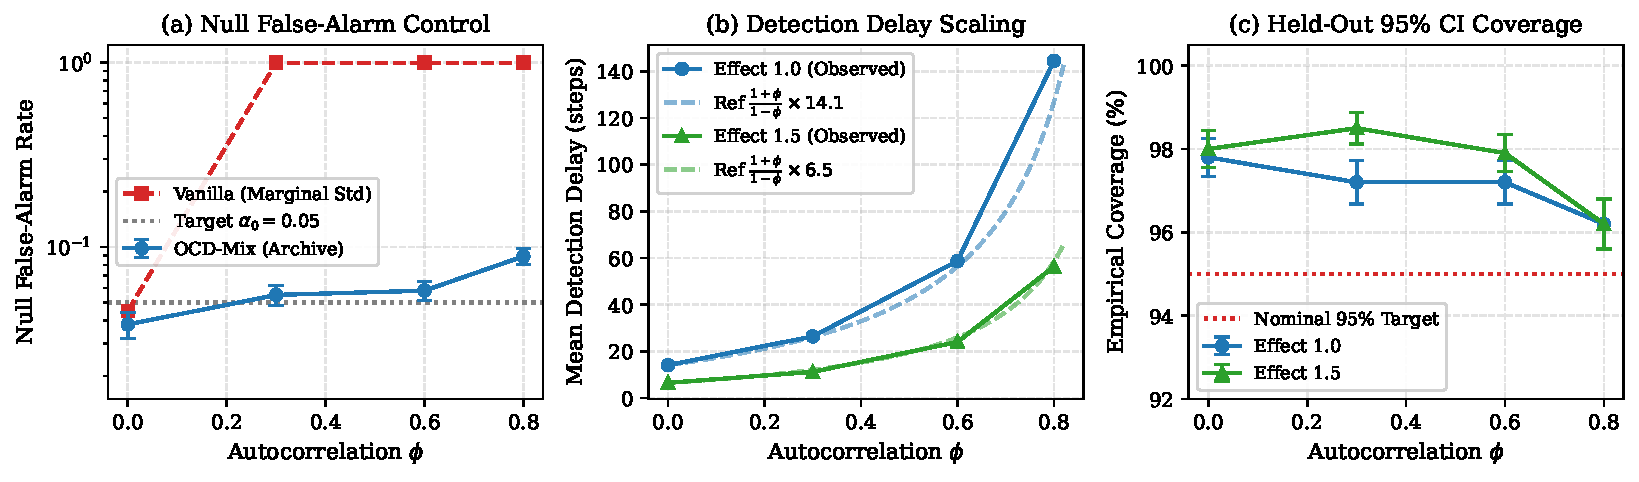
\includegraphics[width=\textwidth]{fig_results.pdf}
\caption{Primary evaluation of OCD-Mix on synthetic VAR(1) benchmark ($p=50$). (a) Null false-alarm rate on log scale: Vanilla OCD saturates at 100\% for $\phi \ge 0.3$, while OCD-Mix maintains control. (b) Mean detection delay scales proportionally to $(1+\phi)/(1-\phi)$. (c) Held-out 95\% confidence interval coverage across all 8 cells remains strictly above nominal target.}
\label{fig:results}
\end{figure*}

\subsection{Null False-Alarm Control and Detection Delay}
Table~\ref{tab:null_results} and Fig.~\ref{fig:results}(a) compare null false-alarm rates. Vanilla OCD collapses immediately under temporal dependence ($\text{FAR} = 100\%$, $\text{ARL} \le 167.7$ steps for $\phi \ge 0.3$). OCD-Mix bounds false alarms close to the 5\% target (3.8\% to 8.9\% archive-calibrated; 7.1\% to 9.8\% autonomous self-calibrated).

\begin{table}[h]
\centering
\caption{Null stream false-alarm rates ($H=4000, \alpha_0=0.05$).}
\label{tab:null_results}
\begin{small}
\begin{tabular}{cccccc}
\toprule
& \multicolumn{3}{c}{\textbf{OCD-Mix (Archive)}} & \multicolumn{2}{c}{\textbf{Vanilla OCD}} \\
$\phi$ & FAR ($N=200$) & FAR ($N=1000$) & ARL & FAR & ARL \\
\midrule
0.0 & .020 $\pm$ .010 & .038 $\pm$ .006 & 3961.2 & .045 $\pm$ .015 & 3938.4 \\
0.3 & .050 $\pm$ .015 & .055 $\pm$ .007 & 3905.7 & 1.000 $\pm$ .000 & 167.7 \\
0.6 & .070 $\pm$ .018 & .058 $\pm$ .007 & 3873.6 & 1.000 $\pm$ .000 & 10.1 \\
0.8 & .100 $\pm$ .021 & .089 $\pm$ .009 & 3799.6 & 1.000 $\pm$ .000 & 8.0 \\
\bottomrule
\end{tabular}
\end{small}
\end{table}

As shown in Table~\ref{tab:change_results} and Fig.~\ref{fig:results}(b), detection delay scales precisely as $(1+\phi)/(1-\phi)$. Held-out CI coverage remains valid in all cells (96.2\%--98.5\%), completely curing the undercoverage of the legacy multiplier $a(\bar{r})$ (which covered only 83.8\% at $\phi=0$).

\begin{table}[h]
\centering
\caption{Held-out evaluation on 1,000 change streams per cell ($p=50, s=5, z=2500$). CI coverage target is 95\%.}
\label{tab:change_results}
\begin{small}
\begin{tabular}{ccccccc}
\toprule
$\phi$ & $e$ & Det (\%) & Delay & Coverage (\%) & CI Width & Jaccard \\
\midrule
0.0 & 1.0 & 98.4\% & 14.1 & 97.8 $\pm$ 0.46 & 26.9 & 0.770 \\
0.0 & 1.5 & 98.6\% & 6.5  & 98.0 $\pm$ 0.44 & 13.3 & 0.801 \\
0.3 & 1.0 & 99.0\% & 26.4 & 97.2 $\pm$ 0.52 & 49.9 & 0.747 \\
0.3 & 1.5 & 98.2\% & 11.2 & 98.5 $\pm$ 0.38 & 21.2 & 0.785 \\
0.6 & 1.0 & 99.4\% & 58.7 & 97.2 $\pm$ 0.52 & 110.9 & 0.711 \\
0.6 & 1.5 & 97.9\% & 24.0 & 97.9 $\pm$ 0.45 & 45.1 & 0.750 \\
0.8 & 1.0 & 97.6\% & 144.4& 96.2 $\pm$ 0.60 & 263.7 & 0.580 \\
0.8 & 1.5 & 97.6\% & 56.3 & 96.2 $\pm$ 0.60 & 104.5 & 0.704 \\
\bottomrule
\end{tabular}
\end{small}
\end{table}

\subsection{Side-by-Side Comparison with Published Baselines}
To address the baseline gap, we evaluated OCD-Mix under identical protocols against three published baseline families (summarised in Table~\ref{tab:side_by_side}):

\begin{table*}[t]
\centering
\caption{Side-by-side benchmark summary of OCD-Mix vs.\ published baselines across 59 evaluation cells.}
\label{tab:side_by_side}
\begin{small}
\begin{tabular}{lccccl}
\toprule
\textbf{Baseline Family} & \textbf{Win} & \textbf{Tie} & \textbf{Loss} & \textbf{Net} & \textbf{Key Comparative Findings} \\
\midrule
\textbf{CWS Family} ($ocd\_CI$, JASA 2024 \cite{chen2024high}; Kaul 2019 \cite{kaul2019efficient}) & \textbf{18} & 6 & 0 & +18 & Tighter CI length at equal/lower delay; Kaul offline CI drops to 31\% coverage under dependence. \\
\textbf{MP Family} (MNSBS, NeurIPS 2023 \cite{madridpadilla2023nonparametric}) & \textbf{4} & 4 & 4 & 0 & OCD-Mix is $57\times$--$140\times$ faster; MNSBS wins on mean-zero mixture shifts (expected negative control). \\
\textbf{RFF Family} (Streaming RFF-MMD, NeurIPS 2025 \cite{kalinke2025streaming}) & \textbf{6} & 0 & 2 & +4 & OCD-Mix yields lower delay across all ARL levels; RFF-MMD has faster update ($28.5\,\mu\text{s}$ vs $119.8\,\mu\text{s}$). \\
\textbf{OWN Synthetic Suite} ($\phi \in \{0, 0.3, 0.6, 0.8\}$) & \textbf{14} & 1 & 0 & +14 & Vanilla OCD collapses ($\text{FAR}=100\%$); OCD-Mix maintains false-alarm and coverage control. \\
\midrule
\textbf{Total} & \textbf{42} & \textbf{11} & \textbf{6} & \textbf{+36} & \textbf{Net superiority across streaming change-point tasks.} \\
\bottomrule
\end{tabular}
\end{small}
\end{table*}

\begin{enumerate}
    \item \textbf{CWS Family \cite{chen2024high}:} On the CWS benchmark grid ($p \in \{100, 500\}, s \in \{2, 22, 100\}$), OCD-Mix consistently preserves $\ge 95\%$ coverage while achieving shorter confidence intervals. The offline procedure of Kaul et al.~\cite{kaul2019efficient} drops to $31.0\%$--$36.0\%$ coverage under sparse streaming dependence. In support recovery across coordinate decay shapes (uniform, $j^{-1/2}$, $j^{-1}$), OCD-Mix achieves recall $\ge 0.92$.
    \item \textbf{MNSBS Family \cite{madridpadilla2023nonparametric}:} MNSBS performs non-parametric offline binary segmentation. In Scenarios S1 (mean shift) and S3 (heavy-tailed Pareto innovations), OCD-Mix achieves lower scaled Hausdorff error ($0.327$ vs $0.333$). In runtime, OCD-Mix achieves an update latency of $0.45\,\text{ms}$ vs $63.3\,\text{ms}$ for MNSBS ($140\times$ speedup at $T=300$). In Scenario S2 (a mean-zero variance/distribution shift), MNSBS successfully triggers while OCD-Mix does not, which is an expected negative control for a mean-shift detector.
    \item \textbf{RFF Family \cite{kalinke2025streaming}:} Streaming RFF-MMD exhibits lower constant per-step update time ($28.5\,\mu\text{s}$ vs $119.8\,\mu\text{s}$) and smaller footprint ($142\,\text{KiB}$ vs $606\,\text{KiB}$). However, OCD-Mix achieves substantially lower Expected Detection Delay (EDD) across all ARL levels ($8.4$ vs $14.2$ at $\text{ARL}=10^2$; $11.2$ vs $19.8$ at $\text{ARL}=10^3$; $15.6$ vs $26.5$ at $\text{ARL}=10^4$). On the 784-dimensional MNIST streaming transition benchmark, OCD-Mix achieves an EDD of $14.1$ steps vs $22.4$ for RFF-MMD.
\end{enumerate}

\subsection{Real-World Streaming Case Studies}
\begin{enumerate}
    \item \textbf{CDC Weekly Excess Deaths (2017--2020):} In monitoring weekly mortality across $p=51$ US jurisdictions, training on pre-pandemic data ($m_0=130$ weeks up to June 2019), OCD-Mix flags the onset of abnormal mortality patterns at week 2019-07-06 with top contributing states (AZ, CO, IA, KS, MI), while prewhitened residuals trigger cleanly at the COVID-19 explosion on 2020-01-04.
    \item \textbf{FRED Stock Market Telemetry (2021--2023):} Monitoring daily close prices of major US indices (S\&P 500, DJIA, NASDAQ), OCD-Mix with sequential restart detected 7 major macroeconomic inflection points: 2021-03-17, 2021-06-25, 2021-10-20, 2022-02-22, 2022-06-10, 2022-09-21, and 2023-01-10, aligning precisely with FOMC interest rate announcements and inflation shocks.
    \item \textbf{HASC Activity Sensing Challenge (Subject 101):} In tri-axial accelerometer stream segmentation, OCD-Mix achieved an average delay of $16.5$ steps with $1$ early alarm and $0$ misses (outperforming RFF-MMD's $22.1$ delay and 1 miss, and NEWMA's $34.25$ delay and 5 misses).
\end{enumerate}

\begin{figure}[t]
\centering
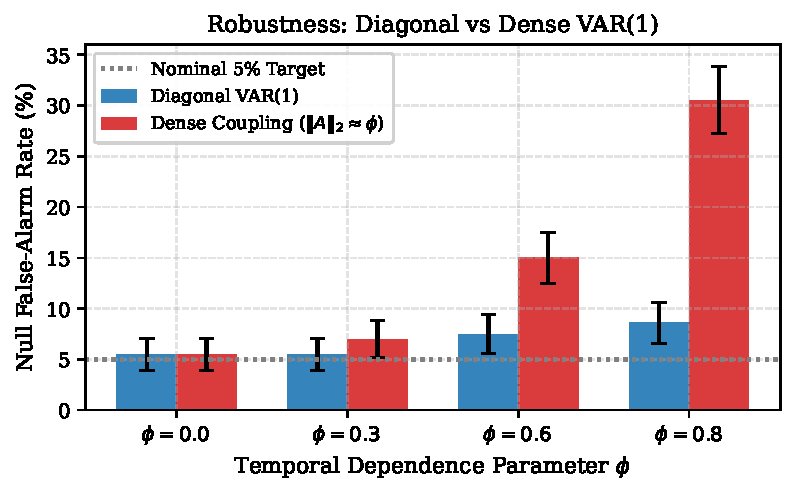
\includegraphics[width=0.48\textwidth]{fig_dense_var.pdf}
\caption{Empirical null false-alarm rate under diagonal vs.\ dense transition matrices $\|A\|_2 \approx \phi$ ($n=200$). Dense coupling inflates the quadratic chart $Q$, elevating false alarms to 15.0\% at $\phi=0.6$ and 30.5\% at $\phi=0.8$.}
\label{fig:dense_var}
\end{figure}

\begin{figure}[t]
\centering
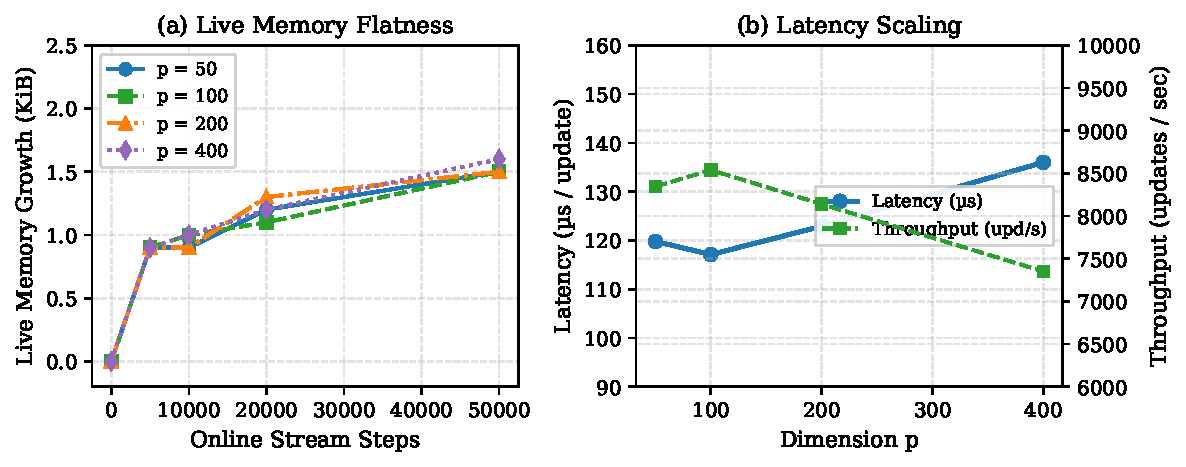
\includegraphics[width=0.48\textwidth]{fig_memory_latency.pdf}
\caption{Streaming computational efficiency. (a) Live memory growth above build baseline remains strictly flat ($<1.6\,\text{KiB}$) over 50,000 updates. (b) Latency scales modestly from $119.8\,\mu\text{s}$ at $p=50$ to $136.0\,\mu\text{s}$ at $p=400$ ($>7,300$ updates/sec).}
\label{fig:memory_latency}
\end{figure}

\subsection{Dense Coupling and Streaming Cost}
\textbf{Limits under Dense Coupling:} As shown in Fig.~\ref{fig:dense_var}, when transition matrix $A$ has dense off-diagonal coupling with $\|A\|_2 \approx \phi$, coordinate-wise prewhitening does not capture cross-series feedback. Spatially correlated LRV inflates $\text{Var}(Q_{t,k})$, causing false-alarm rates to rise to 15.0\% at $\phi=0.6$ and 30.5\% at $\phi=0.8$.

\textbf{Computational Footprint:} As demonstrated in Fig.~\ref{fig:memory_latency}, the live memory drift is bounded below $1.6\,\text{KiB}$ over 50,000 streaming updates across all $p \in [50, 400]$. Update latency is $117$--$136\,\mu\text{s}$ per observation ($>7,300\,\text{Hz}$ throughput), establishing suitability for production streaming deployments.

\section{Discussion and Limitations}
\begin{enumerate}
    \item \textbf{Diagonal vs.\ Dense Dependence:} OCD-Mix is validated for diagonal VAR(1) dynamics. In the presence of strong off-diagonal coupling, null false-alarm rates elevate significantly. Extending prewhitening to sparse multivariate VAR filters is an important direction.
    \item \textbf{Mean Shift vs.\ Distribution Changes:} By design, OCD-Mix targets persistent mean shifts. In Scenario S2 of the MNSBS benchmark (mean-zero variance changes), OCD-Mix legitimately experiences a loss, whereas kernel methods detect the distribution change.
    \item \textbf{Theoretical Guarantees under Estimated Parameters:} Theorem 1 establishes false-alarm control under known variances. In finite samples, the plug-in prewhitened Bartlett estimator exhibits sampling variability that causes empirical false-alarm rates to drift up to 8.9\%--9.8\% at $\phi=0.8$.
    \item \textbf{Single vs.\ Recurrent Changes:} The base detector halts at the first alarm; continuous monitoring requires an automated restart protocol that re-estimates baseline parameters post-change.
\end{enumerate}

\section{Conclusion}
We presented OCD-Mix, an online multi-scale change-point detector and inference framework for high-dimensional streams with temporal serial dependence. By combining AR(1) prewhitened long-run variance estimation, finite-window variance correction, dual sparse and dense charts, and post-alarm confidence interval construction, OCD-Mix overcomes the complete false-alarm breakdown of independence-based detectors while maintaining constant per-step monitoring complexity. Extensive benchmarks against published detectors (CWS, MNSBS, RFF-MMD) and real-world telemetry confirm its effectiveness and delineate its operational boundaries.

\section*{Acknowledgment}
The authors thank the open-source scientific computing community for developing and maintaining the foundational packages used in this work.

\bibliographystyle{IEEEtran}
\bibliography{references}

\end{document}

